\documentclass[aspectratio=169, 12pt, french]{beamer}
\usetheme{AnnArbor}
\usecolortheme{beaver}


% Utilisation de Tikz dans la présention
\usepackage{pgf}
\usepackage{tikz}
\usetikzlibrary{arrows,automata, shapes,chains, positioning, backgrounds}
\tikzstyle{line}=[draw] % here
% Définition d'une flèche
\tikzstyle{arrow} = [thick,->,>=stealth]

% test
\usepackage[comma,authoryear]{natbib}

% tabular environment
\usepackage{tabu} 
\usepackage{xcolor}

% Compatibilité avec Sweave
% ------------------------------------------------------
% Fichier de configuration Sweave
% À utiliser lorsqu'on veut mettre du R au travers de notre rapport R
% Gabriel Crépeault-Cauchon
% fortement inspiré du préambule des documents .TEX à Vincent Goulet
% source : https://gitlab.com/vigou3/programmer-avec-r/blob/master/programmer-avec-r.tex
% ------------------------------------------------------
\usepackage[noae]{Sweave}
\usepackage{framed}                  % env. snugshade*, oframed

\definecolor{midnightblue}{HTML}{dfe3f2} 
%\definecolor{darkred}{rgb}{0.545,0,0} 
%\DefineVerbatimEnvironment{Sinput}{Verbatim}{fontshape=sl,formatcom={\color{midnightblue}}} 
%\DefineVerbatimEnvironment{Scode}{Verbatim}{fontshape=sl,formatcom={\color{blue}}} 
%\DefineVerbatimEnvironment{Soutput}{Verbatim}{formatcom={\color{darkred}}} 

  %% Environnements de Sweave. Les environnements Sinput et Soutput
  %% utilisent Verbatim (de fancyvrb). On les réinitialise pour
  %% enlever la configuration par défaut de Sweave, puis on réduit
  %% l'écart entre les blocs Sinput et Soutput.
  \DefineVerbatimEnvironment{Sinput}{Verbatim}{}
  \DefineVerbatimEnvironment{Soutput}{Verbatim}{}
  \fvset{listparameters={\setlength{\topsep}{0pt}}}
  %% L'environnement Schunk est complètement redéfini en un hybride
  %% des environnements snugshade* et leftbar de framed.sty.
  \makeatletter
  \renewenvironment{Schunk}{%
    \setlength{\topsep}{1pt}
    \def\FrameCommand##1{\hskip\@totalleftmargin
       \vrule width 2pt\colorbox{midnightblue}{\hspace{3pt}##1}%
      % There is no \@totalrightmargin, so:
      \hskip-\linewidth \hskip-\@totalleftmargin \hskip\columnwidth}%
    \MakeFramed {\advance\hsize-\width
      \@totalleftmargin\z@ \linewidth\hsize
      \advance\labelsep\fboxsep
      \@setminipage}%
  }{\par\unskip\@minipagefalse\endMakeFramed}
  \makeatother



% make sure pause does not increase page count
\setbeamertemplate{footline}[frame number]{}

\setbeamertemplate{frametitle continuation}[from second][(suite)]




% Encoding packages
\usepackage[utf8]{inputenc}
\usepackage[T1]{fontenc}
\usepackage{babel}	% Combine with \documentclass[12pt, french]{•}
\usepackage{lmodern}
\addto\captionsfrench{\def\tablename{Tableau}}

% Packages mathématiques / newcommand
\usepackage{amsmath,amsthm,amssymb,latexsym,amsfonts}
\usepackage{empheq}
\usepackage{icomma}
\newcommand{\trainset}{\mathcal{D}_{\mathcal{T}}}
\newcommand{\testset}{\mathcal{D}_{\mathcal{V}}}

% Informations sur la présentation Beamer (Auteur, date, titre, etc.)
\title[\hyperlink{start}{ACT-2101}]{\Large Modélisation statistique d'évènements extrêmes}
\subtitle{\normalsize Application multivariée dynamique aux catastrophes naturelles de l'Océanie}
\author{\large \textbf{Marc-Olivier Ricard}}
\institute{\normalsize Sous la supervision de \\ Marie-Pier Côté}
\logo{
\includegraphics[width=0.15\textwidth]{src/logo_UL.png}} 
\date{\normalsize 4 décembre 2019}


% Options

% Remove navigation symbol
\setbeamertemplate{navigation symbols}{}

%% Style de la bibliographie.
\bibliographystyle{francais}

\frenchbsetup{%
    StandardItemizeEnv=true,       
    ThinSpaceInFrenchNumbers=true, 
    og=«, fg=»                     
  }
 

\begin{document}


\begin{frame}
\titlepage
\end{frame}


\begin{frame}{Plan de la présentation}
\tableofcontents
\end{frame}

\section{Mise en contexte}



\begingroup
\large
\begin{frame}{Motivations}
\begin{itemize}
	\item Intérêt recherche
	\item Stage été 2019
	\item Maîtrise
	\item Problématiques de l'industrie
\end{itemize}
\end{frame}
\endgroup



\section{Notions préliminaires}

\subsection{Théorie classique des valeurs extrêmes}
\begin{frame}{Théorie classique des valeurs extrêmes}
Soit $X_1,\dots, X_n$, une séquence de variables indépendantes, identiquement distribuées et avec fonction de répartition marginale $F$.  \\~\\ \pause
Soit $M_n = \max\{X_1, \dots, X_n\}$, le maximum des $n$ observations. \\~\\ \pause
S'il existe des séquences de constantes $\{a_n > 0\}$ et $\{b_n\}$ tel que $$P\Bigg\{\frac{M_n - b_n}{a_n} \le z \Bigg\}\to G(z), \ \ \  \text{quand} \ \ {n \to \infty}$$ \pause
$G$ appartient à une des distributions de valeur extrême.\\~\\ 
\end{frame}

\begin{frame}{Théorie classique des valeurs extrêmes}
Les trois dernières lois sont les seules distributions limites pour $M^*_n$. \\~\\ \pause
Une meilleure analyse est possible:\\~\\
\structure{Famille de distributions d'extremum généralisée (GEV)}
\begin{equation}  \label{eq:1}
\begin{gathered}
G(z) = \exp \Bigg\{ - \Big[ 1 +\xi\Big(\frac{z-\mu}{\sigma}\Big) \Big]^{-1/\xi}  \Bigg\}
\end{gathered}
\end{equation} 
Trois paramètres: $\mu$ (position), $\sigma$ (échelle), $\xi$ (forme).
\end{frame}

\begin{frame}{Première méthodologie}
\begin{itemize}
\item Les données sont groupées en séquence de longueur $n$. \pause
\item Le maximum de chaque séquence est calculé. \pause
\item Une distribution \textit{GEV} est calibrée à ces maximums. \pause
\item La distribution peut être manipulée.
\end{itemize}
\end{frame}


\subsection{Méthode par l'approche \protect\textit{Peaks over threshold} (POT)}
\begin{frame}{Méthode par l'approche POT}
Soit $X_1,\dots, X_n$. Nous considérons comme évènements extrêmes ceux qui dépassent un certain seuil $u$.\\~\\
Nous savons déjà que $\Pr\{ \max\{X_1,\dots,X_n\} \le z \}\approx G(z)$ (\ref{eq:1}).
\end{frame}

\begin{frame}{Méthode par l'approche POT}
Pour $u$ assez grand, la fonction de répartition de $X-u\ |\ X>u$ est environ
\begin{equation}
H(y) = 1 - \Big(1+\frac{\xi y}{\tilde\sigma}\Big)^{-1/\xi},
\end{equation}
où
\begin{equation*}
{\tilde{\sigma} = \sigma + \xi(u-\mu)}.
\end{equation*} \pause
Famille de distributions \structure{Pareto généralisée}.\\~\\
Paramètres de $H$. 
\end{frame}

\begin{frame}{Deuxième méthodologie}
\begin{itemize}
\item Les données brutes représentent une séquence de valeurs iid  $x_1,\dots,x_n$. \pause
\item Les valeurs extrêmes sont identifiées en définissant un seuil $u$. \pause
\item Les observations qui dépassent $u$ sont définies par $x_{(1)},\dots,x_{(k)}$ et les excès de seuil par $y_j = x_{(j)} - u$. \pause
\item Une distribution Pareto généralisée est calibrée avec les $y_j$. \pause
\item La distribution peut être manipulée.
\end{itemize}
\end{frame}

\begin{frame}{Deuxième méthodologie}
Défi: choix de la valeur du seuil. \\~\\ \pause
Deux méthodes:
\begin{itemize}
\item \textit{Mean residual plot}
\item Estimer les paramètres du modèle pour différents seuils.
\end{itemize}
\end{frame}


\section{Article étudié}

\begin{frame}{Article étudié}
Article choisi: \cite{chavez2016extreme}
\begin{itemize}
\item Récent
\item Longueur et difficulté convenables
\item Sujet spécifique intéressant
\item Implémentation en \textsf{R}
\end{itemize}
\end{frame}

\subsection{Introduction}
\begin{frame}{Introduction}
L'article choisi présente une nouvelle méthodologie....\\~\\  \pause
\begin{itemize}
\item Ce sont les paramètres du modèle choisi qui dépendront des covariables.\pause
\item Améliorer la calibration des lois. 
\item Inférence plus crédible et précise.
\end{itemize}
\end{frame}

\begin{frame}{Introduction}
\begin{itemize}
\item Processus de Poisson non-homogène. \pause
\item Modèles additifs généralisés, splines de lissage et méthode du maximum de vraisemblance pénalisé. \pause
\item Pareto généralisée non-stationnaire. \pause
\item \cite{coles2001introduction}.
\end{itemize}
\end{frame}

\begin{frame}{Critères}
\begin{itemize}
\item Pertes aléatoires encourues à des temps aléatoires. \pause
\item But de l'analyse. \pause
\item Nombre suffisant d'observations. \pause
\item Évènement extrêmes. \pause
\item Covariables significatives. \pause
\item Notes.
\end{itemize}
\end{frame}

\subsection{Approche dynamique de la théorie des valeurs extrêmes}
\begin{frame}{Approche dynamique de la théorie des valeurs extrêmes}
Idée générale du modèle:
\begin{equation*}
g_k(\theta_k) = f_k(x) + h_k(t), \ \ k \in \{1, \dots, p \}
\end{equation*}
où:
\begin{itemize}
\item $\theta$ est le vecteur des $p$ paramètres du modèle,\pause
\item $g_k$ est une fonction de lien, \pause
\item $f_k$ est la fonction pour les différents niveaux d'une variable catégorique, \pause
\item $h_k$ est soit une fonction linéaire paramétrique ou bien une fonction lisse non-paramétrique de $t$.
\end{itemize}
\end{frame}


\begin{frame}{Fréquence}
Le nombre d'excès du seuil $u$ suit un processus de Poisson non-homogène avec comme taux:
 \begin{equation}
 \lambda = \lambda(x, t) = \exp(f_\lambda(x) + h_\lambda(t)).
  \end{equation}
  
%L'application d'un modèle additif généralisé mène à un estimé $\hat\lambda$.
\end{frame}

\begin{frame}{Reparamétrisation}
S'assurer que les procédures de calibration des paramètres $\xi$ et $\beta$ aux données convergent. \\~\\  \pause
Deux paramètres orthogonaux.
\begin{equation*}
 \begin{split}
  \nu = \log((1+\xi)\beta), & \ \xi > -1 \\ 
  \Rightarrow \beta = \frac{\exp(\nu)}{1+\xi}
  \end{split}
  \end{equation*}
\end{frame}

\begin{frame}{Sévérité}
Comme pour $\lambda$, on définit $\xi$ et $\nu$ comme suit:
\begin{equation}\label{eq:8}
 \xi = \xi(x, t) = f_\xi(x) + h_\xi(t)
\end{equation}
  
 \begin{equation}\label{eq:9}
 \nu = \nu(x, t) = f_\nu(x) + h_\nu(t)
 \end{equation}
 
  \begin{equation*}
  \Rightarrow \beta = \beta(x, t) =  \frac{\exp(\nu(x,t))}{1+\xi(x,t)}
 \end{equation*}
\end{frame}

\begin{frame}{Estimation}
Les équations (\ref{eq:8}) et (\ref{eq:9}) sont donc celles qui seront estimées pour être en mesure d'obtenir $\hat\xi$ et $\hat\beta$. \\~\\  \pause
Basés sur les estimateurs $\hat{f}_\xi, \hat{h}_\xi, \hat{f}_\nu$ et $ \hat{h}_\nu$.\\~\\  \pause
Obtenus à partir des vecteurs observés $z_i = (t_i, x_i, {y_t}_{i})$ où:
\begin{itemize}
\item $i \in \{1, \dots, n\}$, \pause
\item $0 \leq t_1 \le \cdots \le t_n \leq T$ représente les temps d'excès de seuil, \pause
\item $x_i$ représente le vecteur des covariables, \pause
\item ${y_t}_{i}$ représente les réalisations ${Y_t}_{i}$, \pause
\item ${Y_t}_{i}$ représente les excès de seuil $u$.
\end{itemize}
\end{frame}

\begin{frame}{Mesures de risque}
\begin{equation}
\widehat{\text{VaR}_\alpha} = u + \frac{\hat\beta}{\hat\xi} \Bigg(\Bigg( \frac{1-\alpha}{\hat\lambda/n'}\Bigg)^{-\hat\xi} -1 \Bigg)
\end{equation} \pause

\begin{equation}
\widehat{\text{ES}_\alpha} =
\begin{cases}
\frac{\widehat{\text{VaR}_\alpha} + \hat\beta + u\hat\xi}{1-\hat\xi}, & \hat{\xi} \in (0,1) \\
\textcolor{red} \infty, & \hat\xi 	\ge 1
\end{cases}
\end{equation} \pause
Plus utile de modéliser directement $\rho = \rho(x, t) = \lambda(x,t)/n'(x, t)$ qui représente le taux d'excès de seuil pour $x$ et $t$.
\end{frame}


%% Application à des données réelles
% le Sweaveopt


\section{Application à des données réelles}

\subsection{Analyse de données}



\begin{frame}{Analyse de données}
Pour mettre en application l'approche proposée par \cite{chavez2016extreme}, deux jeux de données du paquetage \texttt{CASdatasets} sont utilisés. Soit \texttt{auscathist} et \texttt{nzcathist}. \\~\\

Ces données représentent respectivement l'historique des catastrophes naturelles pour l'Australie ainsi que pour la Nouvelle-Zélande. Les prochaines diapositives présentent une analyse globale des données utilisées.
\end{frame}


\begin{frame}
\begin{figure}
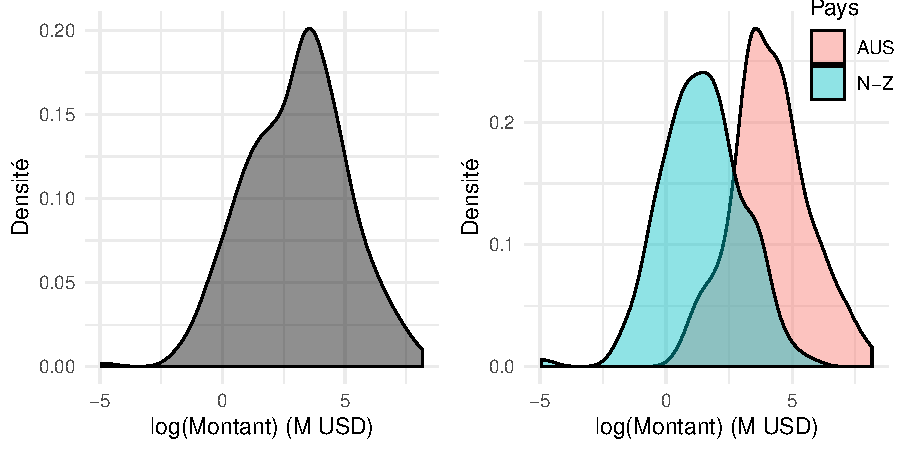
\includegraphics[width=.8\textwidth]{images/fig-005.pdf}
\caption{Densité du logarithme du montant des catastrophes}
\end{figure}
\end{frame}

\begin{frame}
\begin{figure}
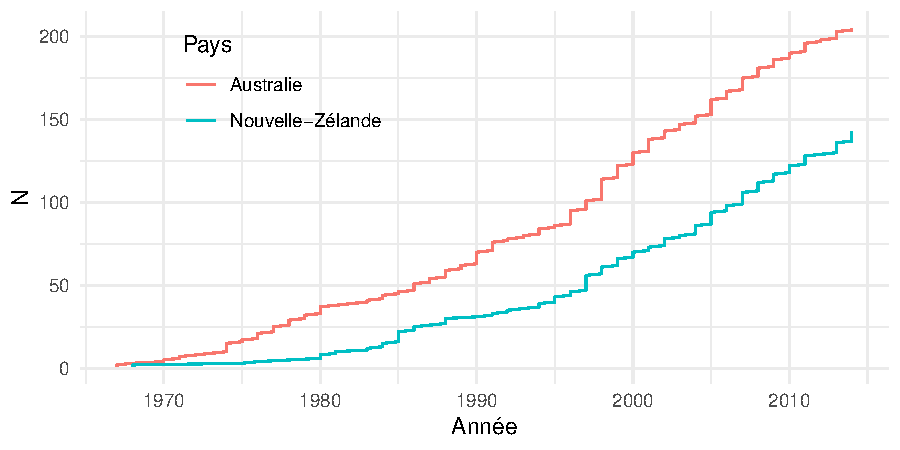
\includegraphics[width=.8\textwidth]{images/fig-006.pdf}
\caption{Nombre cumulatif de catastrophes par pays}
\end{figure}
\end{frame}

\begin{frame}
\begin{figure}
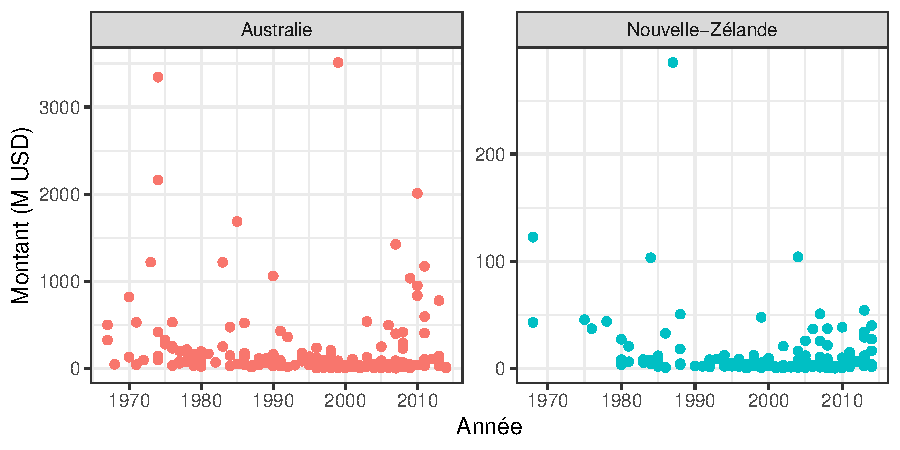
\includegraphics[width=.8\textwidth]{images/fig-007.pdf}
\caption{Évolution des catastrophes par pays}
\end{figure}
\end{frame}

\begin{frame}
% latex table generated in R 3.6.1 by xtable 1.8-4 package
% Mon Nov 25 16:50:46 2019
\begin{table}[ht]
\centering
\begin{tabular}{cccccccc}
  \hline
Type & N & Moyenne & Écart & Minimum & Médiane & Q3 & Maximum \\ 
  \hline
Bushfire & 26 & 143 & 259 & 7 & 39 & 134 & 1217 \\ 
  Cyclone & 37 & 325 & 675 & 2 & 88 & 217 & 3343 \\ 
  Earthquake & 9 & 56 & 91 & 0 & 25 & 47 & 286 \\ 
  Flood & 83 & 62 & 230 & 0 & 5 & 39 & 2010 \\ 
  Flood, Storm & 36 & 54 & 79 & 1 & 24 & 71 & 414 \\ 
  Hailstorm & 41 & 274 & 606 & 0 & 75 & 235 & 3511 \\ 
  Other & 12 & 121 & 296 & 2 & 6 & 50 & 1035 \\ 
  Power outage & 2 & 6 & 6 & 1 & 6 & 8 & 11 \\ 
  Storm & 86 & 97 & 228 & 0 & 28 & 57 & 1424 \\ 
  Tornado & 12 & 7 & 13 & 0 & 3 & 7 & 47 \\ 
  Weather & 4 & 11 & 11 & 2 & 6 & 13 & 27 \\ 
   \hline
\end{tabular}
\caption{Résumé statistique des montants (M USD) de catastrophes par Type} 
\label{tab:3.6}
\end{table}\end{frame}

\subsection{Approche classique}

\begin{frame}
\begin{itemize}
\item Par souci de manque de temps, les résultats obtenus avec l'approche classique ne seront pas montrés de façon détaillée. On conlut que cette approche n'est pas tout à fait adéquate dans le cas présent. 
\item Cette approche reste viable, rapide et peut être une bonne solution lorsque seulement les montants sont disponibles.
\item Un seuil de 10 M USD fut sélectionné
\end{itemize}
\end{frame}



\subsection{Approche dynamique à deux variables}

\subsection{Approche dynamique à trois variables}



\section{Conclusion}
\begin{frame}{Conclusion}
\begin{itemize}
\item Méthode
\item Appréciation
\end{itemize}
\end{frame}


\begin{frame}
\centering
\Huge{\structure{\textbf{Questions?}}}
\end{frame}

\section*{Bibliographie}
\nocite{*}

\begin{frame}[allowframebreaks]{Bibliographie}
\bibliography{biblio}
\end{frame}


\end{document}
